\chapter{Introduction}
\label{ch:ch1}

A Wireless Sensor Network (WSN) is a network of many small, battery-powered 
devices, called motes,  that create ad-hoc networks via wireless radios.  
Motes are inexpensive devices outfitted with various sensors and are configured to 
monitor some phenomena and report back to a server -- called a sink. 
Estrin et al.~\cite{nextCentury} 
elegantly described WSNs as,
\begin{quote}
	``...sensors only interact with other sensors in a restricted 
	vicinity, but nevertheless collectively achieve a desired 
	global objective."
\end{quote}
This captures the essence of a WSN concisely, describing the 
multi-hop environment and how a WSN consists of many small objects 
that are working towards a larger goal.

\begin{figure}[htbp]
	\centering
		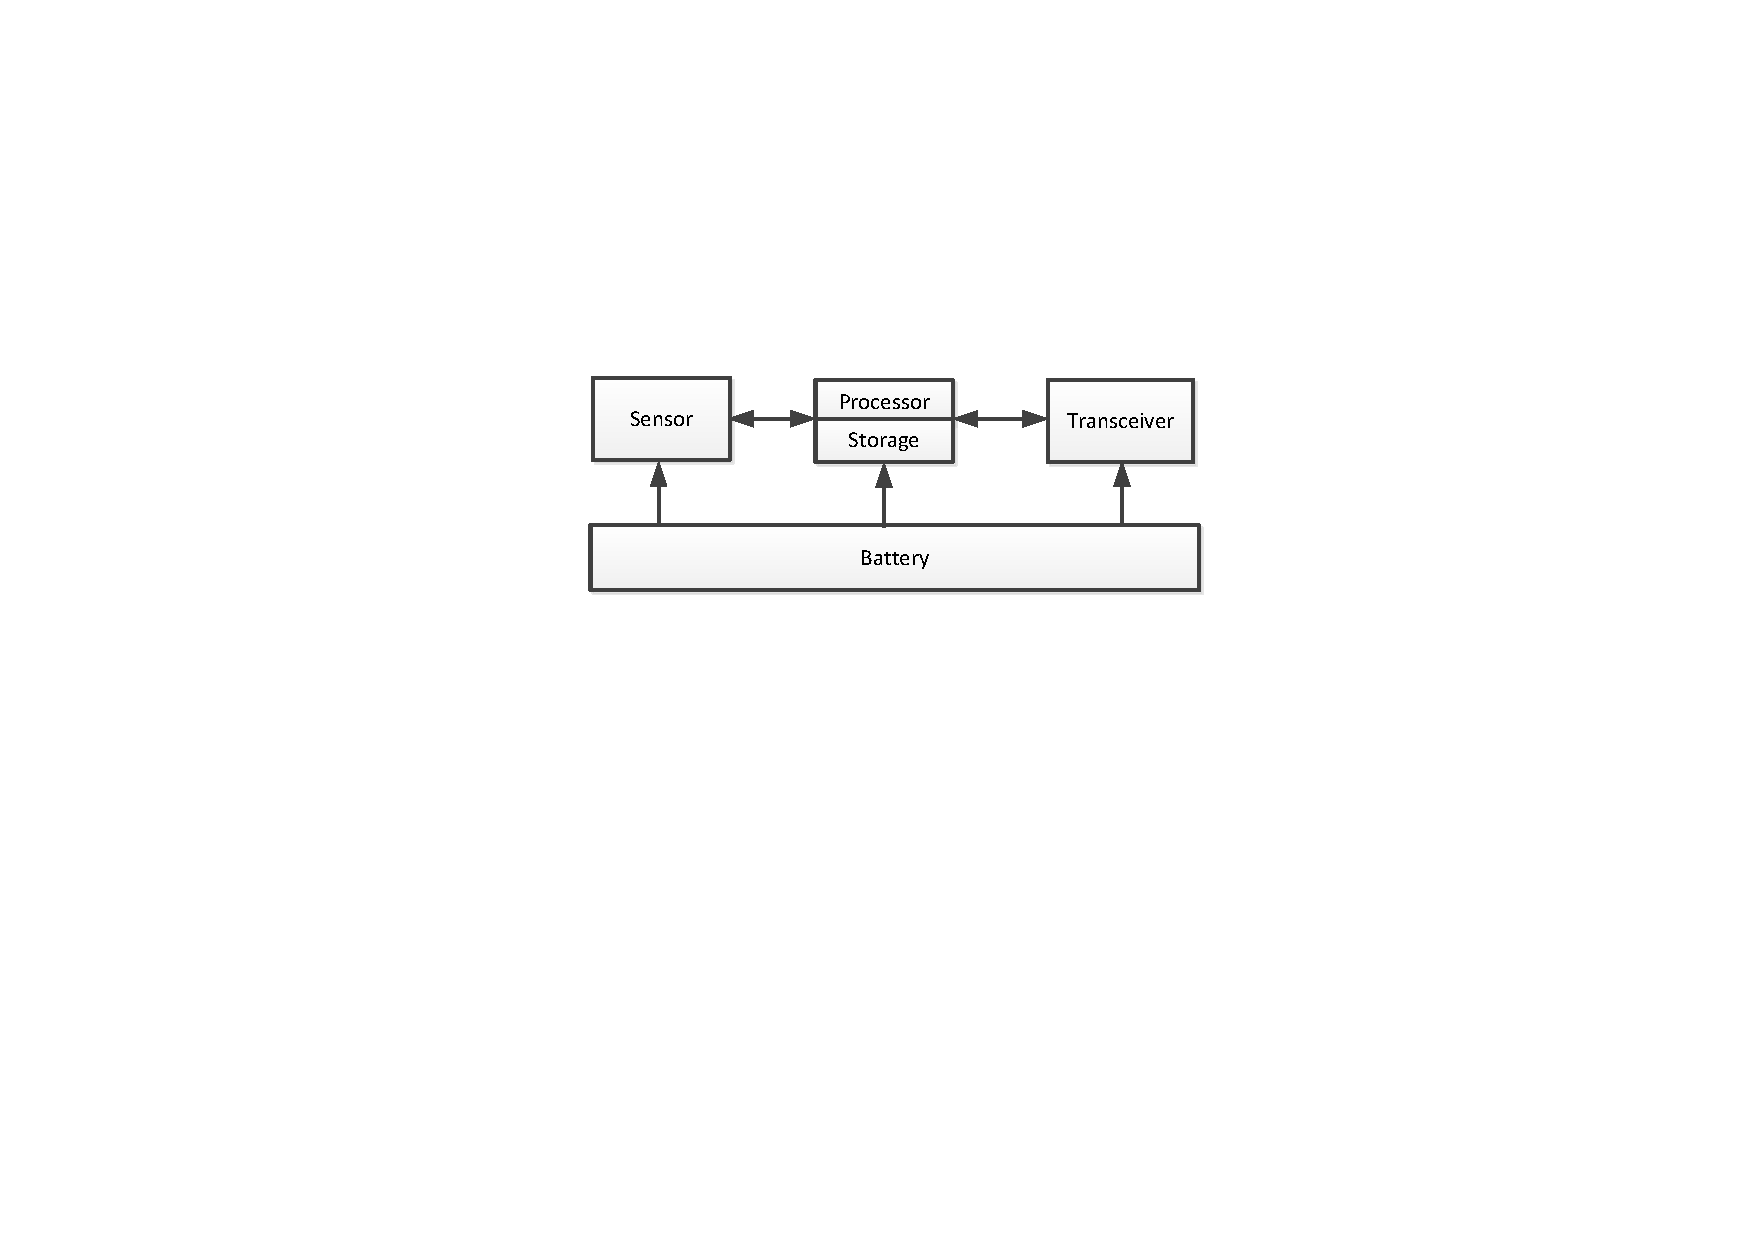
\includegraphics[width=4.5in]{images/intro/mote.pdf}
	\caption{High-level description of a mote. Adapted from ~\cite{wsnSurvey}.}
	\label{fig:images_intro_mote}
\end{figure}

Motes are simple devices that have very few components. 
Motes consist of a battery for power, sensors for
detecting some phenomena, memory for storing the
data collected, a radio for communication and a processor for 
controlling all the other components. Optionally motes
can have ways to regenerate power, such as a solar panel, and 
some motes have the ability to move. The layout of a mote can be seen
graphically in Figure~\ref{fig:images_intro_mote}. 




Applications for WSNs range from animal habitat monitoring~\cite{duckisland,zebranet}
to building and bridge structural monitoring~\cite{StructuralMonitoring}, to 
monitoring live volcanoes during eruptions~\cite{volcano}. 
Typically, when deployed, a WSN self-configures, creating routes from sensor 
motes to the sink automatically. 
Most routes in WSNs are not direct to the sink, therefore motes must use 
several peer motes as a multi-hop network to send messages to the sink.
Routing protocols in WSNs must automatically create these multi-hop routes to 
form a functioning network.
To create these routes, routing algorithms designed for WSNs, such as the
Collection Tree Protocol~\cite{ctp} are used.

There are many scenarios where a WSN could be used to make a task 
simpler, or even save lives.
For instance, Werner-Allen et al.~\cite{volcano} have used a WSN to monitor
a seismic and infrasonic (low-frequency acoustic)  volcanic eruption. The team wanted to have as many motes as possible, and
as long a network lifespan to collect as much data as possible. Every project 
has a limited budget, and high-powered radios are expensive and use lots of energy. 
Since high-powered radios were ruled out, Werner-Allen et al.\ chose to use
a multi-hop WSN. A WSN allowed the team to deploy many sensors with low-power radios 
that could communicate their findings back to the computer they used as a sink. 
Some sensors were lost during the eruption, which could have meant a loss of life or a loss of data
if the sensors required people to continually check them. Since a WSN was
used, the data was transferred off the mote before it was lost to the eruption and provided some
very interesting data!

\begin{wrapfigure}{r}{8cm}
    \fbox{
    \begin{minipage}{7.5 cm}
    
        \begin{center}    
          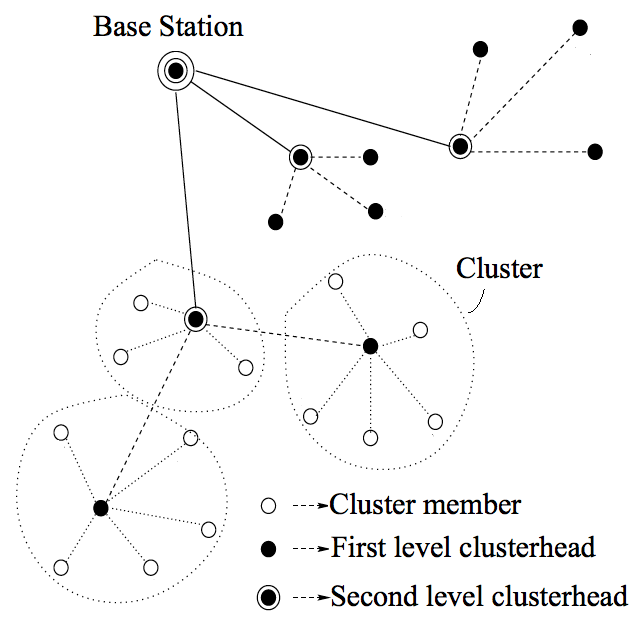
\includegraphics[width=7cm]{images/intro/clusters.png}
        \end{center}
        \caption{A hierarchical cluster topology~\cite{teen}. }
        \label{photo}
    \end{minipage}
    }
  \end{wrapfigure}

WSNs can also be used in less exciting work, such as bridge or vehicle monitoring~\cite{StructuralMonitoring}.
If it is difficult or inconvenient for a person to check strain levels on bridges, a WSN
can be deployed to monitor the bridge. Some of these bridges can be difficult to get power to, as
they might be far into a forest or in a remote location. A battery-powered WSN does not require 
external power to be run to the area, and can continually monitor strain levels without human intervention,
saving companies or governments time and money while making the structure safer.
  
To simplify routing  and to conserve energy, a WSN  groups motes into 
clusters. These clusters elect a clusterhead which works as a gateway and 
routes all network traffic in and out of the cluster. Motes that are cluster 
members only communicate with the clusterhead. Clusterheads then route the 
messages though other clusterheads, to the sink. An example of this can be 
seen in Figure~\ref{photo}.  This simplifies the network topology as each cluster 
can be viewed as one large mote.  Messages to the sink are then routed through 
clusterheads only, which lowers the number of hops taken from the originating 
cluster to the sink. Using clusterheads reduces the energy draw from all motes 
that are in the cluster since they only need to send messages to the 
clusterhead. The clusterhead accepts messages from the motes in the cluster, 
creates one large message out of all the messages, and sends this large 
message to the sink. Handling messages in this way allows motes that are 
cluster members to sleep or be idle while the clusterhead attempts to send the 
message across the network, thus saving power.


A heterogeneous WSN has motes that are not all identical. There may be several 
different types of motes from different companies or motes from the same 
company with different characteristics.  Motes may be running different 
operating systems, be programmed with different software or have additional 
hardware. Homogeneous networks can also be viewed as heterogeneous 
networks; heterogeneity occurs as motes change over time, such as a mote's 
battery depletion or a mote malfunctioning. These differences, large and 
small, can be exploited to extend the network lifespan or increase message throughput.  

In a WSN, typically 
%motes can be specialized to a task to provide more detailed information about the resource it is monitoring.
a mote is assigned to provide detailed information about the phenomenon it is 
monitoring. 
If a few motes are equipped with more expensive hardware, the network should 
adapt to allow these motes to live longer. This can be done by not allowing 
the more expensive mote to be a clusterhead, and by providing a clusterhead 
in range of the expensive mote.
As this specialization increases, so does the heterogeneity of the network. 
Clusterheads should be selected to allow the specialized motes to have  
longer lifespans. Or, if a mote has a larger available message queue it should be
elected to be a clusterhead since it will be less likely to lose messages
if a large number of messages are sent to it, making the mote a good message routing mote.

% redundant?
%The network must be aware of the resources to each mote and select clusterheads within radio range of these motes. In a highly specialized heterogeneous network, clusterheads must be chosen to allow all the specialized motes to communicate with the sink to ensure both network lifetime is long and messages from the motes get to the sink.

A `long-lived WSN' is a network that is designed to stay active for extended 
periods of time. Long-lived WSNs use techniques such as duty cycling and make 
as few transmissions as possible to achieve longer network lifespan. It is 
difficult to have a long-lived network mostly due to the battery-powered 
nature of motes. Long-lived networks often trade off some functionality, such 
as the frequency of sampling with their sensors and the frequency of 
reporting,  to increase mote lifespan.

A clusterhead is a mote that controls transmissions from other 
motes in the immediate neighbourhood. Clusterhead motes draw more power due to 
the increased number of transmissions they perform as they must stay active to receive messages 
from the cluster. 
The key to long-lived networks is selecting motes that are well-suited to be clusterheads.  
Therefore, in a 
heterogeneous long-lived WSN, motes that have more or larger batteries and have plenty 
of residual energy should be elected to be clusterheads. If the 
clusterhead has little power left or has a malfunctioning radio, the 
probability of losing messages increases. Using heterogeneity to avoid 
choosing a mote that is better designed to be a clusterhead will aid in 
designing a long-lived network.

Suitable clusterheads are important when building a long-lived WSN. The 
clusterhead draws a large amount of power, therefore  the performance of 
clusterhead motes will degrade over time. If a clusterhead mote detects that 
it is performing poorly (e.g., cannot keep up handling the incoming messages 
from their motes), it should opt-out or demote itself to pass the task on to a 
more capable mote. Passing the clusterhead task to a more capable mote will 
prevent the poorly-performing mote from losing transmissions and causing 
retransmissions, which creates unnecessary overhead in the surrounding motes.

To increase message throughput, extend lifespans of individual motes and allow WSNs to function longer, I 
have developed Heterogeneous Clustering and Control Protocol (HCCP). HCCP 
uses a taxonomy to describe heterogeneity and selects candidate clusterheads 
based on the capabilities of motes.



